El enunciado presenta el problema de hallar el camino entre 2 puntos que se pueda recorrer en el menor tiempo posible, dandonos un escenario en donde los caminos presentan paredes que podemos atravezar rompiendolas, teniendo a la vez, una determinada cantidad de rupturas a poder realizar. La solución buscada será entre todos los caminos posibles desde el origen al destino, el que resulte mínimo.

Cada camino esta compuesto de unas unidades "caminables", que las llamaremos baldozas. Ir de una baldoza a otra consume la misma cantidad de tiempo en todos los casos. Por otro lado, hay 
baldozas que demandan romper una pared para ser caminadas, con lo cual el camino que se esta transitando debe gastar 1 unidad de esfuerzo en romperla, factor que no influye en el tiempo del recorrido.

Si caracterizamos cada baldoza con un nodo, y la posibilidad de ir de una baldoza a otra como una arista, entonces podemos modelar el problema con un grafo. Como el factor tiempo es constante en cada traslado entre baldozas, las aristas tendrán todas el mismo peso.

A partir de este grafo, sacar el camino mínimo del nodo origen al destino se puede realizar utilizando el algoritmo de busqueda por anchura. El cual permite saber la distancia (o tiempo) a la que se encuentra determinado nodo con cada uno de los demas. De aplicarlo sobre la estructura propuesta en forma directa, se obtendrían soluciones invalidálidas, ya que es necesario tener en cuenta la restricción de cantidad de paredes posibles para romper. También se puede ver que el algoritmo solo, no considera todos los posibles caminos válidos hacia el destino, por lo cual se pierden soluciones v\'alidas al restringir el uso de cada nodo a 1 solo camino:

  \vspace*{0.3cm} \vspace*{0.3cm}
  \begin{center}
 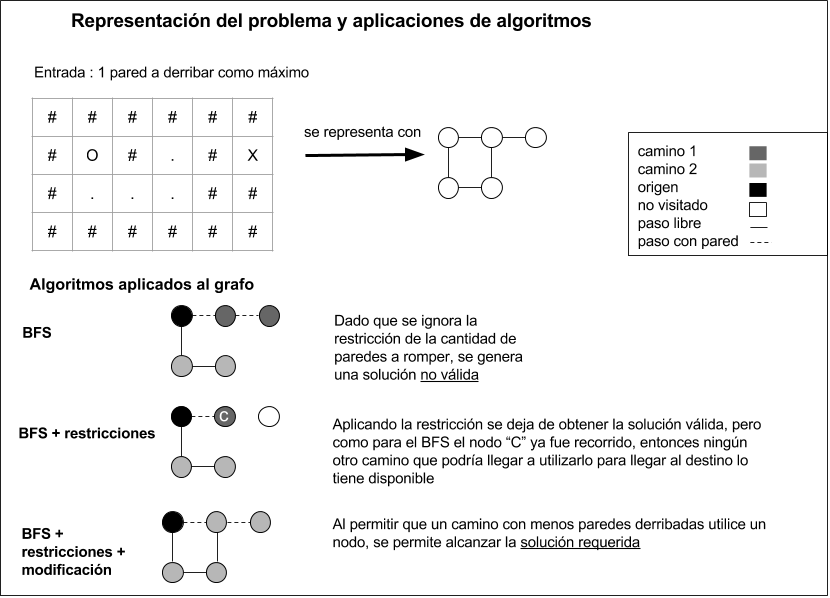
\includegraphics[scale=0.6]{./EJ1/ej1-explicacion.png}
  \end{center}
  \vspace*{0.3cm}

Para poder calcular todos los caminos que pueden llegar efectivamente al destino, en cada nodo se guardará las caracteristicas del tiempo y de las paredes necesarias para alcanzarlo:
\begin{itemize}
\item Si no ha sido alcanzado, entonces, se guarda el tiempo y las paredes necesarias para llegar a \'el.
\item Si ya ha sido alcanzado, entonces si la cantidad de paredes rotas hasta llegar hasta él por el camino actual es menor a la cantidad de paredes que fueron rotas anteriormente, entonces se considera que el camino actual es la mejor forma de alcanzar al nuevo nodo, actualizando los datos del camino actual en el nodo.
\item En el caso de que alcanzar al nodo previamente visitado, demande el mismo tiempo y esfuerzo que en el camino actual, se desestima el camino actual.
\item Si el nodo a evaluar es el destino, se da por finalizado el algoritmo y se devuelve el estado del camino que lo alcanzó.
\end{itemize}